\providecommand\ExamFontPath{../../../字体/}
\documentclass[fontset=exam]{exam-zh}
\usepackage{longtable,booktabs,array,calc,multirow,fvextra}
\usepackage[normalem]{ulem}
\providecommand{\hl}[1]{#1}
\providecommand{\ul}[1]{\uline{#1}}
\DefineVerbatimEnvironment{verbatim}{Verbatim}{breaklines=true,fontsize=\small}
\providecommand{\tightlist}{\setlength{\itemsep}{0pt}\setlength{\parskip}{0pt}}
\newcommand{\pandocbounded}[1]{#1}
\setlength{\emergencystretch}{3em}
\setlength{\tabcolsep}{2pt}
\examsetup{page/size=a4paper}
\title{厦门大学 2009 年 期末考试 A 卷}
\subject[4em]{离散数学}
\begin{document}
\maketitle
\fancyfoot[C]{第 \thepage 页（共 \pageref*{LastPage} 页）}
\begin{enumerate}
\item
  选择题（共 15 题，每题 2 分，共 30 分）
\end{enumerate}

1．下列语句不是命题的有（ ）。

A．x=13。\\
B．离散数学是计算机系的一门必修课。\\
C．鸡有三只脚。\\
D．太阳系以外的星球上有生物。

2．设 p：天下大雨，q：小王乘公共汽车上班，命题``只有天下大雨，小王才乘公共汽车上班''的符号化形式为（ ）。

A．p\(\to\)q B．q\(\to\)p　　C．p\(\to\) \(\neg\)q D． \(\neg\)p\(\to\)q

3．谓词公式\(\left. \exists x(P(x) \vee \forall yR(y))\rightarrow Q(x) \right.\)中的\(x\)( )。\\
A．只是约束变元。\\
B．只是自由变元。\\
C．既非约束变元又非自由变元。\\
D．既是约束变元又是自由变元。

4. 下面式子中，（ ）是不正确的。

A.\(\left. \forall x(A(x) \land B(x))\Leftrightarrow\forall xA(x) \land \forall xB(x) \right.\)\\
B.\(\left. \exists x(A(x) \vee B(x))\Leftrightarrow\exists xA(x) \vee \exists xB(x) \right.\)\\
C.\(\left. \exists x(A(x)\rightarrow B)\Leftrightarrow\exists xA(x)\rightarrow B \right.\)\\
D.\(\left. \forall x(A\rightarrow B(x))\Leftrightarrow A\rightarrow\forall xB(x) \right.\)

5．设个体域为整数集合，则下列公式中真值为 1 的是( )。

A．\(\forall\)x\(\forall\)y(x + y = 1)。 B．\(\forall\)x\(\exists\)y(x + y = 1)。\\
C．\(\exists\)x\(\forall\)y(x + y = 1)。 D．\(\neg\) \(\exists\)x\(\exists\)y(x + y = 1)。

6．下列命题为假的是( )。

A．\{\(\varnothing\)\}\(\in\) P(\(\varnothing\)) B．\(\varnothing\) \(\subseteq\) P(\{\(\varnothing\)\}) C．\{\(\varnothing\)\} \(\supseteq\) P(\(\varnothing\)) D．P(\(\varnothing\)) \(\in\)P(\{\(\varnothing\)\})

7．下列关于集合的势的叙述中，（ ）是错误的。

A. 实数集比自然数集优势。\\
B. 任一无限集合都存在与自己等势的真子集。\\
C. 集合类上的优势关系是偏序关系。\\
D. 有理数集比整数集优势。

8．设\(A,B,C\)是集合，\(F\)是关系，则下列式子中不正确的是（ ）。

A．\(\left. A - B = \varphi\Leftrightarrow A \cup B = B \right.\) B. \(\left. (A \oplus B) = (A \oplus C)\Leftrightarrow B = C \right.\)\\
C. \(F\lbrack A \cap B\rbrack = F\lbrack A\rbrack \cap F\lbrack B\rbrack\) D. \((A \oplus B) \oplus C = A \oplus (B \oplus C)\)

9．设 A=\{1,2,3,\ldots,100\}，R 是 A 上相等关系``=''，由 R 产生等价类有（ ）。

A．10 个　 B．50 个　 C．100 个　 D．1 个

10．集合 A=\{1，2，3，4\}上的偏序关系 R 的关系图为

\begin{quote}
\par\medskip{\centering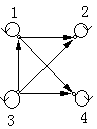
\includegraphics[width=5cm,height=4cm,keepaspectratio]{figures/image14.png}\par}\medskip
\end{quote}

则它的哈斯图为（ ）。

\par\medskip{\centering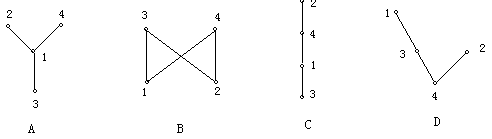
\includegraphics[width=5cm,height=4cm,keepaspectratio]{figures/image15.png}\par}\medskip

11．下列关系中能构成函数的是（ ）。

A．\(\{ < x,y > |(x,y \in N) \land (x + y < 10)\}\) B．\(\{ < x,y > |(x,y \in R) \land (y = x^{2})\}\)\\
C．\(\{ < x,y > |(x,y \in R) \land (y^{2} = x)\}\) D．\(\{ < x,y > |(x,y \in Z) \land (x \equiv y\;mod3)\}\)

12．\(N\)是自然数集，定义\(\left. f:N\rightarrow N,f(x) = (x)mod3 \right.\)（即\(x\)除以 3 的余数），则\(f\)是（ ）。

A．满射不是单射 B．单射不是满射 C．双射 D．不是单射也不是满射

13．设 R 为实数集，定义*运算如下：a*b=\textbar a+b+ab\textbar，则*运算满足（ ）。

A．结合律 B．交换律　　C．有幺元 D．幂等律

14. 数的乘法在下列集合中不封闭的有（ ）。

A．\(\{ 0,1\}\) B．\(\{ x\left| {x\text{为素数}\}} \right.\) C.\(\{ a\sqrt{2} + b\left| {a,b \in Z\}} \right.\) D．\(\{ x\left| {x \in C\text{且}|x|} \right. = 1\}\)

15．下图所示的哈斯图所表示的偏序集中不是格的是（ ）。

\par\medskip{\centering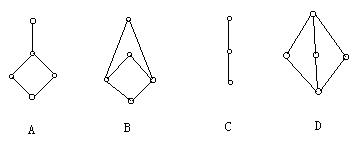
\includegraphics[width=5cm,height=4cm,keepaspectratio]{figures/image28.jpeg}\par}\medskip

\pdfbookmark[1]{二、填空题（共10空，每空2分，共20分）}{section33}

\par\medskip{\heiti

二、填空题（共 10 空，每空 2 分，共 20 分）

\par}\smallskip

1．命题 \(\varnothing\) \(\subseteq\) \{\{\emph{a}\}\} \(\subseteq\) \{\{\emph{a}\},3,4,1\} 的真值 = \underline{\hspace{2cm}}。\\
2．已知集合 A=\{\(\varnothing\),1,2\}，则 A 的幂集 P(A) =\underline{\hspace{2cm}}。\\
3．含 n 个命题变项的重言式的主合取范式为\underline{\hspace{2cm}}。\\
4．设集合 A=\{a,b,c,d \}，则 A 上的不同的等价关系共有\underline{\hspace{2cm}}个，A 上有\underline{\hspace{2cm}}个不同的双射函数。\\
5．设 B 为布尔代数，a,b,c\(\in\)B，则((a\(\land\)b)\(\land\)(a\(\lor\)c))\(\lor\)a 的化简式为\underline{\hspace{2cm}}。\\
6. 设 F(x):x 是人，H(x,y):x 与 y 一样高，在一阶逻辑中，命题``人都不一样高''的符号化形式为\ul{\underline{\hspace{2cm}}}。\\
7． 公式\(\left. \forall x(P(x)\rightarrow Q(x,y)) \vee \exists z(R(y,z)\rightarrow S(x)) \right.\)的自由变元是 ，约束变元是 。\\
8．设\(A\)=\{\textless1,2\textgreater,\textless2,4 \textgreater,\textless3,3\textgreater\} , \(B\)=\{\textless1,3\textgreater,\textless2,4\textgreater,\textless4,2\textgreater\},则\(A \circ B\)= 。

\pdfbookmark[1]{三、计算题（每题5分，共15分）}{section35}

\par\medskip{\heiti

三、计算题（每题 5 分，共 15 分）

\par}\smallskip

1．（5 分）求命题公式\(\left. (\neg p\rightarrow(p \vee r)) \land (p\leftrightarrow q) \right.\)的主析取范式。\\
2．（5 分）设集合 A=\{a，b，c，d\}，A 上的关系 R=\{\textless a，a\textgreater,\textless a，b\textgreater,\textless b，a\textgreater,\textless c，d\textgreater,\textless b，c\textgreater\} 求：\\
（1）画出 R 的关系图。(1 分)\\
（2）R 的自反闭包、对称闭包和传递闭包的关系图。（1 分，1 分和 2 分）

3.（5 分）设\textless A,R\textgreater 为一偏序集，其中 A=\{1，2，3，4，6，8，12，24\}，R 是 A 上的整除关系。\\
（1）画出偏序集\textless A,R\textgreater 的哈斯图。（3 分）\\
（2）求 A 的极大元和极小元。（1 分）\\
（3）求 B=\{2,3,6\}的最小上界和最大下界。（1 分）

\pdfbookmark[1]{四、简答题（共10分）}{section38}

\par\medskip{\heiti

四、简答题（共 10 分）

\par}\smallskip

1．（4 分）设解释 R 如下：D\textsubscript{R}是实数集，D\textsubscript{R}中特定元素 a=0，D\textsubscript{R}中特定函数\(f(x,y) = x - y\)，特定谓词\(F(x,y):x < y\)，问公式\(\left. A = \forall x\forall y\forall z(F(x,y)\rightarrow F(f(x,z),f(y,z))) \right.\)的涵义如何？（2 分）真值如何？（2 分）

2．（6 分）判断下列公式是否是永真式？并说明理由。

(1) (\(\exists\)\emph{xA}(\emph{x})\(\to\)\(\exists\)\emph{xB}(\emph{x}))\(\to\)\(\exists\)\emph{x}(\emph{A}(\emph{x})\(\to\)\emph{B}(\emph{x}))。（3 分）

(2) (\(\forall\)\emph{xA}(\emph{x})\(\to\)\(\forall\)\emph{xB}(\emph{x}))\(\to\)\(\forall\)\emph{x}(\emph{A}(\emph{x})\(\to\)\emph{B}(\emph{x})))。（3 分）

\pdfbookmark[1]{五、证明题（共25分）}{section43}

\par\medskip{\heiti

五、证明题（共 25 分）

\par}\smallskip

1．（10 分）

（1）（5 分）在命题逻辑的自然推理系统中构造下面推理的证明。

前提：\(\neg\)(P\(\land\)\(\neg\)Q)，\(\neg\)Q\(\lor\)R，\(\neg\)R

结论：\(\neg\)P

（2）（5 分）在谓词逻辑的自然推理系统中构造下面推理的证明。

前提：\(\forall\)x（\(\neg\)A（x）\(\to\)B（x）），\(\forall\)x \(\neg\)B（x）

\begin{quote}
结论：\(\exists\)x A（x）
\end{quote}

2．（5 分）叙述并证明容斥原理。（2 分和 3 分）

3．（5 分）设\emph{R}是集合\emph{A}上的一个具有传递和自反性质的关系，\emph{T}是\emph{A}上的关系，使得

\emph{\textless a，b\textgreater{}\(\in\)T\(\Leftrightarrow\)\textless a，b\textgreater{}\(\in\)R 且\textless b，a\textgreater{}\(\in\)R}，证明\emph{T}是一个等价关系。

4．（5 分）设\(< B, \land , \vee ,',0,1 >\)是布尔代数，\emph{a,b}\(\in\)\emph{B}，试证\(a = b\text{当且仅当}(a \land b') \vee (a' \land b) = 0\)。

六 应用题（该题为附加题，8 分）

甲、乙、丙、丁 4 个人有且仅有 2 个人参加围棋优胜比赛。关于谁参加竞赛，下列 4 种判断都是正确的：

(1)甲和乙只有一人参加；

(2)丙参加，丁必参加；

(3)乙或丁至多参加一人；

(4)丁不参加，甲也不会参加。

请推出哪两个人参加了围棋比赛。

\end{document}
